\documentclass[Bachelorarbeit.tex]{subfiles}
\begin{document}
\chapter{Entwicklung}
In der Planungsphase werden allgemeine Überlegung zu der Umsetzung 
des Projektes getätigt, die anschließend bewertet und im Kapitel 
\nameref{chap:implementierung} realisiert werden. Da die Hardwarekomponenten definiert wurden 
behandeln das folgende Kapitel ausschließlich die Lösungsansätze 
beziehungsweise Dokumentationen der Softwarekomponenten.

\section{Überlegungen zur Softwarearchitektur}
Zum aktuellen Stand kann die Software in vier Aufgabenbereiche aufgeteilt werden: 
Steuerung, Kommunikation, Domäne und Persistenz. Das Steuerungs-Modul bildet zum einem
den zentralen Einstiegspunkt in das Programm, anderem delegiert es Aufgaben an die 
entsprechenden Stellen. Für die Kommunikation mit den Energiezählern ist das 
Kommunikations-Modul verantwortlich. In der Domäne werden die zu 
überwachenden Energiezähler und ihre Messwerte verwaltet. Für die Speicherung 
der Daten dient das Persistenz-Modul.\\
%
Um einem gewissen Maß an Flexibilität zur gewährleisten sowie um Änderungen  
beziehungsweise spätere Erweiterungen zu ermöglichen, ist es von Vorteil wenn die einzelnen Schichten so weit wie möglich entkoppelt werden. 
Darunter versteht man, dass es für die einzelnen Schichten unerheblich ist, von welcher Quelle sie ihre Informationen und Befehlsdelegationen erhalten und jene somit leichter austauschbar sind. \\
%
Um die Wartbarkeit und Effizienz des Quellcodes zu maximieren 
sollte schon bei der Modellierung auf ein hohes Maß an Kohäsion geachtet 
werden. Unter Kohäsion versteht man, wie effektiv die einzelnen 
Strukturen ausschließlich ihren definierten Aufgabenbereich abdecken. Dies 
bedeutet anhand eines "`bildlichen Beispiels"' demonstriert: die Struktur 
Personalbüro die Operationen „Person einstellen“ und „Person entlassen“ 
anbietet, nicht aber die Operation „Kundendaten anlegen“. 
Durch ein hohes Maß an Kohäsion wird der Code-Verdopplung vorgebeugt und 
der Anteil des wiederverwendbaren Quelltext maximiert. \\

\subsection{Entwurf des Modells }
Nachdem die einzelnen Schichten - auf der Basis ihrer Kompetenz-Bereiche - definiert wurden, liegt der nächste Schritt in der Überlegung wie die Interaktion der Schichten untereinander umgesetzt werden können. 
An dieser Stelle werden die verschiedenen Entwürfe, die im Entwicklungsprozess optimiert wurden, vorgestellt. 

\subsubsection*{Erster Entwurf}
Aktuell wird von dem zentralen Steuerungs-Modul aus eine neue Kommunikation initiiert. Zum besseren Verständnis des allgemeinem Kommunikationsablaufes dient das Flussdiagramm im Anhang A (siehe Abb.: \ref{pic:flussdiagramm_kommunikation}). \\
Die Steuerung ruft das Modul für die Modbus-Kommunikation auf und übergibt die für die 
Kommunikation benötigten Daten.  Das Kommunikationsmodul 
verwertet die erhaltenen Daten, um die Kommunikation zum gewünschten 
Energiezähler aufzubauen und sendet das erzeugte Modbus-Frame. \\
Grundsätzlich können während der Kommunikation zwei verschiedene Fälle eintreten. 
Der optimale Fall wäre es wenn die Kommunikation ohne Fehler abläuft. 
Dabei wurden die ausgelesenen Daten von dem Kommunikationsmodul an die Steuerung weitergegeben (\textit{Case1}). 
Das alternative Szenario wäre es, das bei der Kommunikation ein Fehler aufgetreten ist (\textit{Case2}). Sollte Case2 eingetreten entstehen zwei weitere Ablaufverhalten. 
Je nach Fehlerquelle kann entweder versucht werden, die Kommunikation erneut aufzubauen (\textit{Case2.1}), oder die Kommunikation wird endgültig abgebrochen (\textit{Case2.2}).
Im Falle eines Abbruches wird ein spezifischer Fehlercode retourniert. 
Nach dem Erhalt der Daten leitet das Steuer-Modul die Informationen an das Kommunikations-Modul weiter, um sie schlussendlich in einer geeigneten Struktur abzulegen\footnote{Bei der aktuellen Planung werden nur Daten bei erfolgreicher Kommunikation gespeichert, dies entspricht ausschließlich \textit{Case1} und \textit{Case2.1}.}\\\\
Aus diesem Ansatz wurde folgendes Schichtenmodell entworfen. (siehe Abb.: \ref{pic:schicht_zentral})\\
\begin{figure}
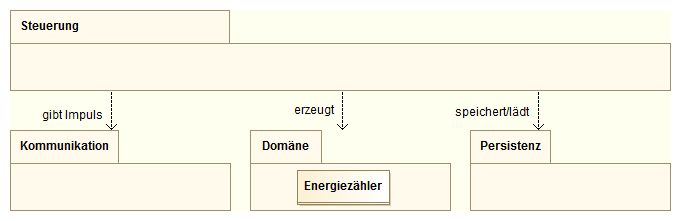
\includegraphics[width=0.9\textwidth]{./img/Schichtenarchitektur_zentralisiert.png}
\caption{Schichtenmodell mit zentralen Ansatz}
\label{pic:schicht_zentral}
\end{figure}

\subsubsection*{Optimierter Entwurf}
Bei dem aktuellen Entwurf (siehe Abb.: \ref{pic:schicht_zentral}) geht jede Interaktion von dem Steuerungs-Modul aus. Die einzelnen Module (untere Schicht) müssen für die Operationen allerding nicht das Steuerungs-Modul (obere Schicht) kennen, man spricht von einer einseitigen 
Abhängigkeit. Wenn die Module über wohldefinierte Schnittstellen verfügen, ist auch 
der - zuvor erwähnte - Austausch von Modulen möglich, wodurch eine Entkopplung 
der Schichten stattfindet. Durch die Entkopplung der Schichten wurde ein weiteres
Konzept der Schichtenarchitektur - die Zugriffsvirtualisierung – realisiert. Der zentrale 
Ansatz muss nicht vollständig verworfen werden, allerdings sollten gewisse Stellen 
überarbeitet werden. \\
Wie zuvor erwähnt, bildet die Domäne die zu verwaltenden Energiezähler ab. 
Dies bedeutet, die gemessenen Werte gehören zu jeweils einem speziellen Zähler. 
Die hardwarespezifischen Information für den Auslesevorgang, wie zum Beispiel über welche Adresse oder 
welche Befehlssätze der Zähler verfügt, besitzt jeder Energiezähler selbst.  Die Wissenskompetenz liegt dementsprechend bei dem
Energiezähler beziehungsweise seiner Instanziierung aus der Domäne. 
Von dieser Annahme ausgehend, wäre es sinnvoll – sowie der Kohäsion dienlich – wenn ein Energiezähler (Instanziierung eines \\
Domänenobjektes) selbst über einen eigenen geräte-spezifischen Befehlssatz und die entsprechenden Verbindungsinformationen verfügt. 
Aus diesen Änderungen würde folgendes neues Schichtenmodell entstehen (siehe Abb.: \ref{pic:schicht_optimiert})\\
\begin{figure}[h]
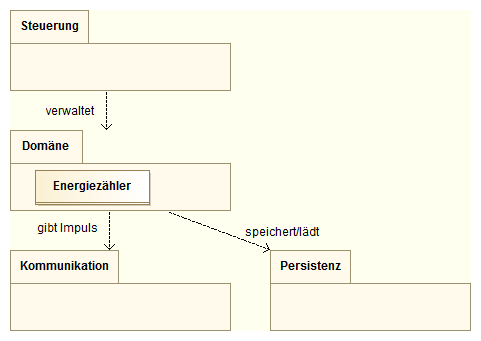
\includegraphics[width=0.75\textwidth]{./img/Schichtenarchitektur_optimiert.png}
\caption{überarbeitetes Schichtenmodell}
\label{pic:schicht_optimiert}
\end{figure}
\\
Die neue Version des Modells (siehe Abb.: \ref{pic:schicht_optimiert}) weist nun die Eigenschaften von 
einseitigen Abhängigkeiten zwischen den Schichten sowie einer realisierten 
Zugriffsvirtualisierung\footnote{Entkopplung zwischen den einzelnen Schichten} auf. Das überarbeitete Modell kann dem Konzept der 
Schichtenarchitektur zugeordnet werden.
\end{document}
